\documentclass{article}
\usepackage[utf8]{inputenc}
\usepackage{amsmath}
\usepackage{graphicx}
\usepackage{caption}
\usepackage[toc,page]{appendix}
\usepackage{float}

\usepackage{listings}
\usepackage{color} %red, green, blue, yellow, cyan, magenta, black, white
\definecolor{mygreen}{RGB}{28,172,0} % color values Red, Green, Blue
\definecolor{mylilas}{RGB}{170,55,241}



\title{Praktische Foutenschatters d.m.v. Nulregels}
\author{Peter Coppens \\ In Samenwerking Met: Alexander Boucquey, Simon Dirckx, Cédric Picron}
\date{}

\setlength\parindent{0pt}

\graphicspath{{./figs/}}

\begin{document}

\lstset{language=Matlab,%
    %basicstyle=\color{red},
    breaklines=true,%
    morekeywords={matlab2tikz},
    keywordstyle=\color{blue},%
    morekeywords=[2]{1}, keywordstyle=[2]{\color{black}},
    identifierstyle=\color{black},%
    stringstyle=\color{mylilas},
    commentstyle=\color{mygreen},%
    showstringspaces=false,%without this there will be a symbol in the places where there is a space
    numbers=left,%
    numberstyle={\tiny \color{black}},% size of the numbers
    numbersep=9pt, % this defines how far the numbers are from the text
    emph=[1]{for,end,break},emphstyle=[1]\color{red}, %some words to emphasise
    %emph=[2]{word1,word2}, emphstyle=[2]{style},    
}

\maketitle

\section{Trapezium regel}
We gebruiken de samengestelde regel beschreven in (Numerical approximation of integrals). Om dan de trapezium regel te implementeren, nemen we $w_j = \left\{1, 1\right\}$, $x_j = \left\{-1, 1\right\}$. \\

Deze implementatie geeft de relatieve errors: \\
$f_1: 0.123355$ \\
$f_2: 0.032950$ \\
$f_3: 0.033711$ \\
$f_4: 0.033461$. \\

De grootte van deze fouten kan intuitief verklaard worden aan de hand van figuur~\ref{fig:ctrap}.

\begin{figure}[H]
\centering
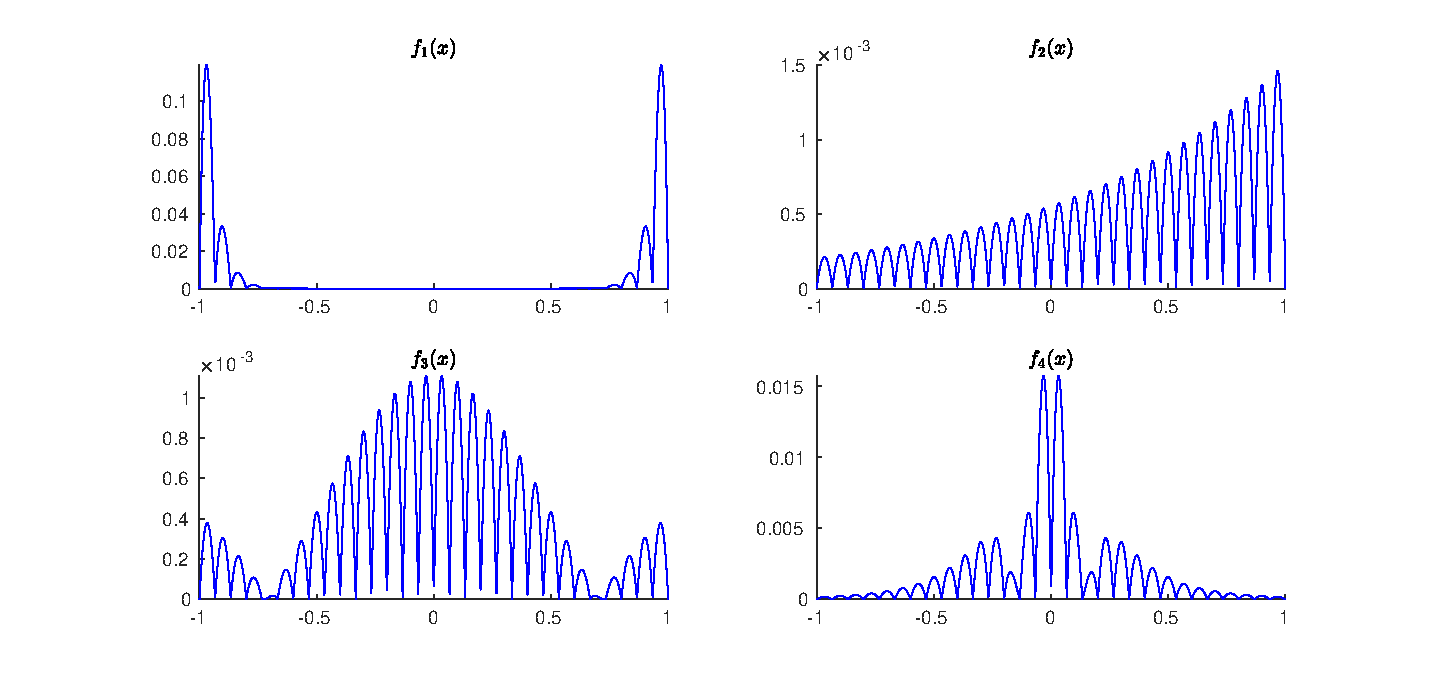
\includegraphics[width=\linewidth, trim=2cm 0.5cm 2cm 0.5cm, clip]{ctrap.eps}
\caption{Error between interpolation by trapezium rule and the actual function.} \label{fig:ctrap}
\end{figure}

\section{Nulregels}
We berekenen de nulregels a.d.h.v de momentvergelijking op p237. We gaan dus niet uit van symmetrische regels (aangezien dit niet gevraagd is in de opgave). Een overgang naar deze zou echter wel de nauwkeurigheid verhogen. We berekenen nulregelse gebaseerd op $n+1 = 31$ punten. Deze willen we even sterk maken als de trapezium regel. We doen dit aan de hand van de MATLAB code in Appendix~\ref{s:nm}. De input is dan de vector berekend door de code in Appendix~\ref{s:ctrap}. \\

De berekende errors $e_j$ worden weergegeven in figuur~\ref{fig:e}. De errors $E_j$ na het verwijderen van het fase-effect worden getoond in figuur~\ref{fig:E}.

\begin{figure}[H]
\centering
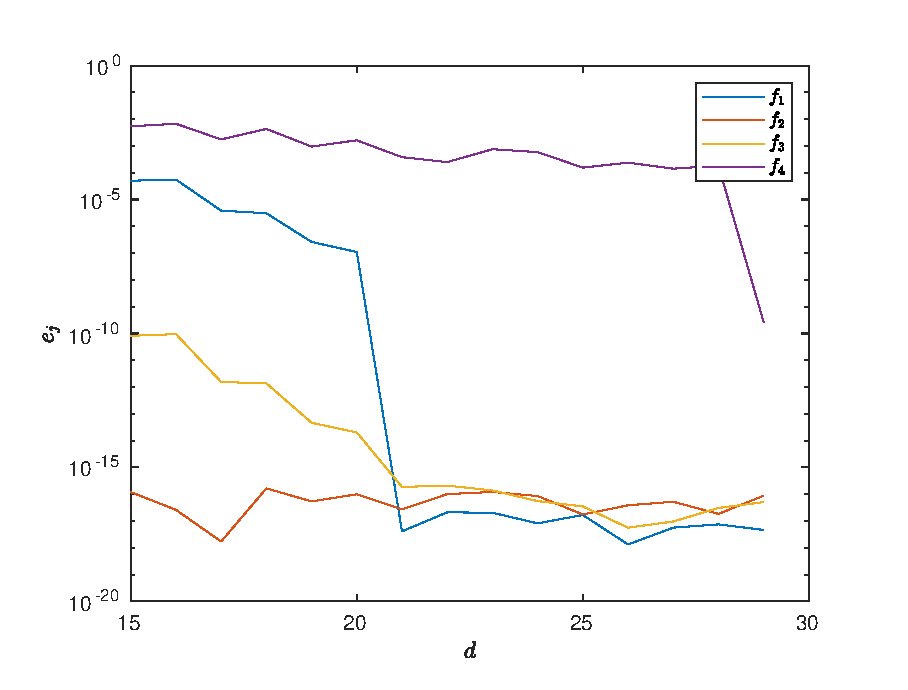
\includegraphics[width=\linewidth]{e.eps}
\caption{$e_j$ in functie van de graad van de nulregel.} \label{fig:e}
\end{figure}

\begin{figure}[H]
\centering
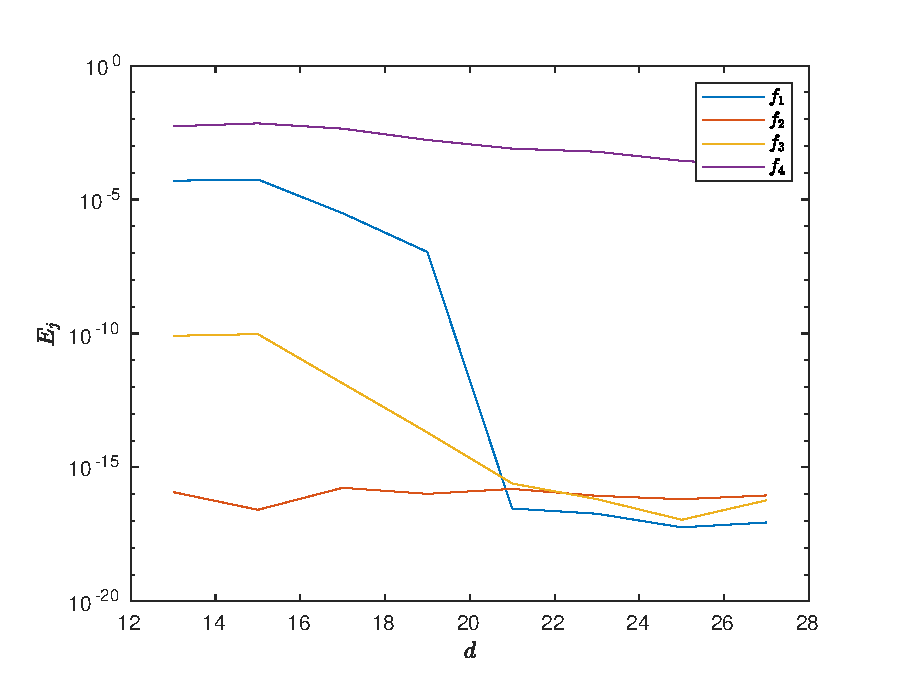
\includegraphics[width=\linewidth]{E.eps}
\caption{$E_j$ in functie van de graad van de nulregel.} \label{fig:E}
\end{figure}

\section{Reductie factoren}
Bij het berekenen van de factoren zullen we de errors $e_j$, die rond machine precisie liggen, uitsluiten. Ze bestaan namelijk hoofdzakelijk uit ruis van de berekeningen. We beschouwen een error als ruis als: $e_j < 10^{-10}$, in dit geval kiezen we $r_j = 10^{-10}$ (in de rest van de berekeningen zouden deze dan niet gebruikt moeten worden, maar dit maakt de plots wel duidelijker).

Figuur~\ref{fig:R} toont twee plots. De bovenste is van de reductie factoren $r_j$ voor het verwijderen van de fase effecten. De onderste is die van $R_j$ na het verwijderen van de fase effecten. \\

Merk op dat de lage waarden die afwisselend optreden bij $e_j$ zijn uitgevlakt bij $E_j$. Dit wordt dan ook zichtbaar als men $r_j$ en $R_j$ vergelijkt.\\

We zien sterke convergentie bij $f_1$ en $f_3$. Ze zitten echter in het ruis gebied, waardoor dit niet te bevestigen valt aan de hand van de reductie factoren. $f_1$ gaat duidelijk naar het asymptotisch gebied, voordat hij eveneens in het ruis gebied terecht komt. $f_4$ blijft de hele tijd zwak asymptotisch.


\begin{figure}[H]
\centering
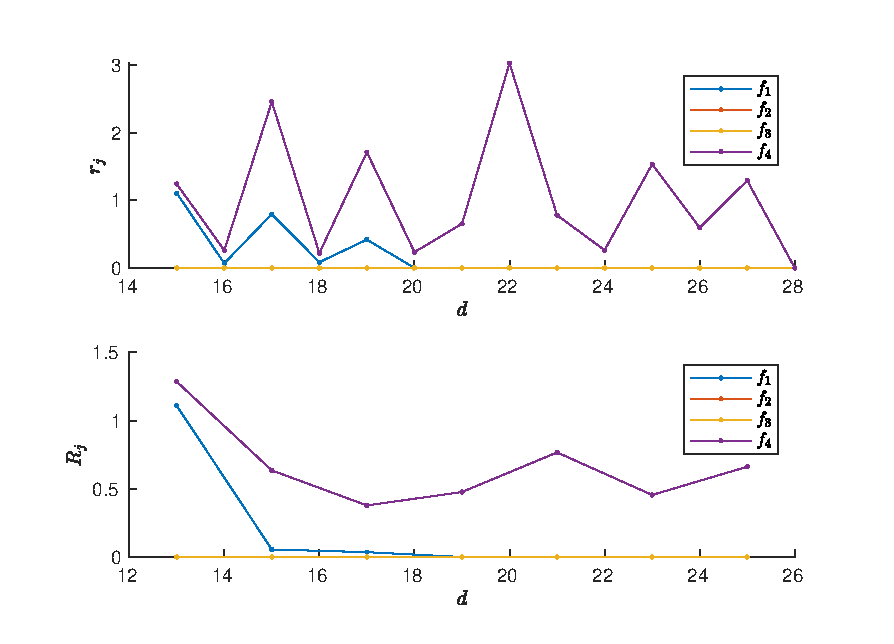
\includegraphics[width=0.95\linewidth]{R.eps}
\caption{Reductie factoren, met en zonder fase effect.} \label{fig:R}
\end{figure}

\section{Foutenschatting}
We kunnen de nulregels, bepaald in de eerdere secties niet gebruiken om de fout op de samengestelde trapezium regel te bepalen. Dit is namelijk geen interpolerende regel van $n+1=31$ punten. De theorie gaat ervan uit dat dit wel het geval is. Voor de samengestelde trapezium regel kunnen we maar één nulregel bepalen: $n = \left[-0.5, 0.5\right]$. Deze moet dan toegepast worden op elk deelinterval waar we de normale trapezium regel op toepassen om een lokale fouten schatting te krijgen. Dit doen we aan de hand van het eerste algoithm in Sectie 6 van de tekst over nulregels. Dit is uitgewerkt in MATLAB code in Appendix~\ref{s:qag}. We bekomen de schatting: \\
$f_1: \quad 0.0333$ \\
$f_2: \quad 0.5614$ \\
$f_3: \quad 0.0211$ \\
$f_4: \quad 0.0314$ \\
De werkelijke fout is: \\
$f_1: \quad 0.0117$ \\
$f_2: \quad 0.0774$ \\
$f_3: \quad 0.0504$ \\
$f_4: \quad 0.0222$ \\
Merk op dat de schatting een redelijke bovengrens is voor $f_1$ en $f_4$, een extreme bovengrens voor $f_2$ en onder de fout zit voor $f_3$.
Dit zijn geen geweldige resultaten.

\pagebreak
\begin{appendices}
\section{Code om de samengestelde trapezium regel te berekenen.} \label{s:ctrap}
\lstinputlisting{ctrap.m}
\pagebreak
\section{Code om de nulregels te berekenen} \label{s:nm}
\lstinputlisting{null_moment.m}
\pagebreak
\section{Code voor QAG algorithm} \label{s:qag}
\lstinputlisting{qag.m}
\end{appendices}

\end{document}
